\chapter{IMPLEMENTATION DETAILS}

\section{Lexical Analyser}

The lexical analyser is implemented in \texttt{components/lexica.py} as the class \texttt{PropLogicLexer}, extending \texttt{sly.Lexer}. It converts an input string into a stream of tokens using regular expression pattern matching.

\begin{lstlisting}[caption={Token definitions in \texttt{PropLogicLexer}}, label={lst:lexer}]
class PropLogicLexer(Lexer):
    tokens = { TRUE, FALSE, AND, OR, LPAREN, RPAREN }

    ignore = ' \t'

    AND    = r'[∧&]'
    OR     = r'[∨|]'
    LPAREN = r'\('
    RPAREN = r'\)'
    TRUE   = r't'
    FALSE  = r'f'

    def error(self, t):
        bad = t.value[0]
        self.index += 1
        raise ValueError(
            f"Illegal character '{bad}' "
            f"at position {self.index}")
\end{lstlisting}

\textbf{Key design choices:}
\begin{itemize}
    \item Both Unicode ($\wedge$, $\vee$) and ASCII (\texttt{\&}, \texttt{|}) operators are accepted via character class regex patterns.
    \item The \texttt{ignore} attribute silently consumes whitespace.
    \item The \texttt{error()} method raises a \texttt{ValueError} with a message identifying the illegal character and its position.  This exception propagates up to the GUI, which displays the error to the user.
\end{itemize}

\textbf{Tokenisation example.} For the input \texttt{t $\vee$ f $\wedge$ f}, the lexer produces the token stream shown in Table~\ref{table:tokenisation}.

\begin{table}[H]
\centering
\caption{Tokenisation of \texttt{t $\vee$ f $\wedge$ f}}
\label{table:tokenisation}
\begin{tabular}{@{}cccc@{}}
\toprule
Position & Character & Token Type & Token Value \\
\midrule
0 & \texttt{t}       & \texttt{TRUE}  & \texttt{t} \\
2 & $\vee$           & \texttt{OR}    & $\vee$ \\
4 & \texttt{f}       & \texttt{FALSE} & \texttt{f} \\
6 & $\wedge$         & \texttt{AND}   & $\wedge$ \\
8 & \texttt{f}       & \texttt{FALSE} & \texttt{f} \\
\bottomrule
\end{tabular}
\end{table}

Whitespace at positions 1, 3, 5, and 7 is consumed by the \texttt{ignore} directive.

\section{Parser --- LALR(1)}

The parser is implemented in \texttt{components/parsers.py} as the class \texttt{PropLogicParser}, extending \texttt{sly.Parser}. It uses the \textbf{LALR(1)} (Look-Ahead Left-to-right Rightmost-derivation) parsing algorithm~\citep{aho2006compilers}.

\subsection{LALR(1) Parsing Algorithm}

LALR(1) is a \textbf{bottom-up} parsing algorithm that reads input left to right, produces a rightmost derivation in reverse, and uses one token of lookahead~\citep{aho2006compilers}.  It operates via a \textbf{shift-reduce} mechanism: \emph{shift} pushes the next token onto the parse stack, while \emph{reduce} replaces a sequence matching a production's right-hand side with the corresponding non-terminal, executing the associated semantic action (AST node construction).  Parsing runs in $O(n)$ time with respect to input length, and the SLY library automatically generates the LALR(1) parse table from the grammar rules and precedence declarations.

\subsection{Precedence Declaration}

\begin{lstlisting}[caption={Precedence declaration in \texttt{PropLogicParser}}, label={lst:precedence}]
precedence = (
    ('left', OR),      # Level 1 - lower priority
    ('left', AND),     # Level 2 - higher priority
)
\end{lstlisting}

In SLY, tokens listed \textbf{later} in the precedence tuple bind \textbf{tighter}. This ensures that $\wedge$ has higher precedence than $\vee$. When a shift/reduce conflict arises, the parser compares the precedence of the lookahead token with the precedence of the reduction rule and chooses accordingly.

\subsection{Grammar Rules with Semantic Actions}

Each grammar rule is implemented as a decorated method that constructs the corresponding AST node:

\begin{lstlisting}[caption={Grammar rules with semantic actions}, label={lst:grammar_rules}]
@_('expr OR expr')
def expr(self, p) -> Expression:
    return Expression_logic(Operations.OR, p.expr0, p.expr1)

@_('expr AND expr')
def expr(self, p) -> Expression:
    return Expression_logic(Operations.AND, p.expr0, p.expr1)

@_('LPAREN expr RPAREN')
def expr(self, p) -> Expression:
    return p.expr

@_('TRUE')
def expr(self, p) -> Expression:
    return Expression_bool(True)

@_('FALSE')
def expr(self, p) -> Expression:
    return Expression_bool(False)
\end{lstlisting}

The semantic actions are \textbf{syntax-directed}: each grammar rule directly constructs the corresponding AST node, building the tree bottom-up as reductions occur during parsing.

\subsection{Parsing Trace}

Table~\ref{table:parse_trace} shows the step-by-step LALR(1) shift-reduce parsing process for the input \texttt{t $\vee$ f $\wedge$ f}, demonstrating how precedence resolves the ambiguity.

\begin{table}[H]
\centering
\caption{LALR(1) shift-reduce parsing trace for \texttt{t $\vee$ f $\wedge$ f}}
\label{table:parse_trace}
\begin{tabular}{@{}clllp{4.5cm}@{}}
\toprule
Step & Stack & Input & Action & Semantic Action \\
\midrule
1  & ---                        & \texttt{t $\vee$ f $\wedge$ f} & Shift \texttt{t}     & --- \\
2  & \texttt{TRUE}              & \texttt{$\vee$ f $\wedge$ f}   & Reduce (5) & \texttt{Expression\_bool(True)} \\
3  & \texttt{expr}              & \texttt{$\vee$ f $\wedge$ f}   & Shift $\vee$       & --- \\
4  & \texttt{expr $\vee$}       & \texttt{f $\wedge$ f}          & Shift \texttt{f}     & --- \\
5  & \texttt{expr $\vee$ FALSE} & \texttt{$\wedge$ f}            & Reduce (6) & \texttt{Expression\_bool(False)} \\
6  & \texttt{expr $\vee$ expr}  & \texttt{$\wedge$ f}            & Shift $\wedge$ $^*$ & --- \\
7  & \texttt{expr $\vee$ expr $\wedge$} & \texttt{f}             & Shift \texttt{f}     & --- \\
8  & \texttt{expr $\vee$ expr $\wedge$ FALSE} & ---               & Reduce (6) & \texttt{Expression\_bool(False)} \\
9  & \texttt{expr $\vee$ expr $\wedge$ expr}  & ---               & Reduce (3) & \texttt{Expression\_logic(AND, \ldots)} \\
10 & \texttt{expr $\vee$ expr}  & ---                             & Reduce (2) & \texttt{Expression\_logic(OR, \ldots)} \\
11 & \texttt{statement}         & ---                             & Accept     & Return root AST node \\
\bottomrule
\end{tabular}
\end{table}

$^*$ At step 6, a \textbf{shift/reduce conflict} occurs: the parser could either reduce \texttt{expr $\vee$ expr} by rule (2) or shift $\wedge$. Because AND has \textbf{higher precedence} than OR, the parser chooses to \textbf{shift}, correctly binding $\wedge$ tighter.


\section{Abstract Syntax Tree (AST)}

The AST is implemented in \texttt{components/ast/statement.py} using an inheritance hierarchy of three classes. Figure~\ref{fig:class_hierarchy} shows the class structure.

\begin{figure}[H]
\centering
\begin{tikzpicture}[
    class/.style={rectangle, draw=black, thick, rounded corners=3pt,
                  minimum width=3.2cm, minimum height=0.9cm,
                  text centered, font=\small\bfseries},
    arrow/.style={-{Stealth[length=5pt]}, thick},
    node distance=1.5cm
]
\node[class, fill=boxblue]   (base)  {Expression (ABC)};
\node[class, fill=boxgreen, below left=1.5cm and 0.3cm of base]  (bool)  {Expression\_bool};
\node[class, fill=boxorange, below right=1.5cm and 0.3cm of base] (logic) {Expression\_logic};

\draw[arrow] (bool.north)  -- (base.south west);
\draw[arrow] (logic.north) -- (base.south east);

\node[font=\scriptsize, below=0.1cm of bool, text width=3cm, align=center]
    {Leaf node\\(truth value)};
\node[font=\scriptsize, below=0.1cm of logic, text width=3cm, align=center]
    {Binary node\\(logical operation)};
\end{tikzpicture}
\caption{AST class hierarchy}
\label{fig:class_hierarchy}
\end{figure}

Table~\ref{table:ast_classes} summarises each class.

\begin{table}[H]
\centering
\caption{AST node classes}
\label{table:ast_classes}
\begin{tabular}{@{}lllp{5cm}@{}}
\toprule
Class & Role & Fields & Key Methods \\
\midrule
\texttt{Expression}      & Abstract base class & \texttt{value}   & \texttt{run()}, \texttt{prefix()} (abstract) \\
\texttt{Expression\_bool} & Leaf: truth literal  & \texttt{value: bool}   & \texttt{run()} $\rightarrow$ \texttt{bool}; \texttt{prefix()} $\rightarrow$ \texttt{"t"} or \texttt{"f"} \\
\texttt{Expression\_logic} & Binary: logical op  & \texttt{operation}, \texttt{left}, \texttt{right} & \texttt{run()} $\rightarrow$ recursive eval; \texttt{prefix()} $\rightarrow$ prefix string \\
\bottomrule
\end{tabular}
\end{table}

The \texttt{Operations} enum defines the two operations:

\begin{lstlisting}[caption={\texttt{Operations} enum}, label={lst:operations}]
class Operations(Enum):
    AND = 0
    OR  = 1
\end{lstlisting}

\subsection{AST Construction Example --- Parse Tree}

For the input expression \texttt{t $\vee$ f $\wedge$ f}, the parser constructs the AST shown in Figure~\ref{fig:ast_example}. This tree is the direct result of the LALR(1) parsing process described in Table~\ref{table:parse_trace}.

\begin{figure}[H]
\centering
\begin{tikzpicture}[
    level distance=1.8cm,
    sibling distance=3.5cm,
    treenode/.style={circle, draw=black, thick, minimum size=1cm,
                     font=\small\bfseries, inner sep=2pt},
    leaf/.style={rectangle, draw=black, thick, rounded corners=2pt,
                 minimum width=1cm, minimum height=0.7cm,
                 font=\small\bfseries, inner sep=4pt},
    edge from parent/.style={draw, thick, -{Stealth[length=4pt]}}
]
\node[treenode, fill=boxorange] {$\vee$}
    child { node[leaf, fill=boxgreen] {\texttt{t}}
        edge from parent node[left, font=\scriptsize] {left}
    }
    child { node[treenode, fill=boxorange] {$\wedge$}
        child { node[leaf, fill=boxred] {\texttt{f}}
            edge from parent node[left, font=\scriptsize] {left}
        }
        child { node[leaf, fill=boxred] {\texttt{f}}
            edge from parent node[right, font=\scriptsize] {right}
        }
        edge from parent node[right, font=\scriptsize] {right}
    };
\end{tikzpicture}
\caption{AST (parse tree) for \texttt{t $\vee$ f $\wedge$ f} --- $\wedge$ binds tighter and forms a subtree under $\vee$}
\label{fig:ast_example}
\end{figure}

Figure~\ref{fig:ast_paren} shows the AST for the parenthesised expression \texttt{(t $\vee$ f) $\wedge$ f}, where parentheses override the default precedence.

\begin{figure}[H]
\centering
\begin{tikzpicture}[
    level distance=1.8cm,
    sibling distance=3.5cm,
    treenode/.style={circle, draw=black, thick, minimum size=1cm,
                     font=\small\bfseries, inner sep=2pt},
    leaf/.style={rectangle, draw=black, thick, rounded corners=2pt,
                 minimum width=1cm, minimum height=0.7cm,
                 font=\small\bfseries, inner sep=4pt},
    edge from parent/.style={draw, thick, -{Stealth[length=4pt]}}
]
\node[treenode, fill=boxorange] {$\wedge$}
    child { node[treenode, fill=boxorange] {$\vee$}
        child { node[leaf, fill=boxgreen] {\texttt{t}}
            edge from parent node[left, font=\scriptsize] {left}
        }
        child { node[leaf, fill=boxred] {\texttt{f}}
            edge from parent node[right, font=\scriptsize] {right}
        }
        edge from parent node[left, font=\scriptsize] {left}
    }
    child { node[leaf, fill=boxred] {\texttt{f}}
        edge from parent node[right, font=\scriptsize] {right}
    };
\end{tikzpicture}
\caption{AST (parse tree) for \texttt{(t $\vee$ f) $\wedge$ f} --- parentheses force $\vee$ to be evaluated first}
\label{fig:ast_paren}
\end{figure}


\section{Evaluation --- Truth Value Computation}

The \texttt{run()} method evaluates the AST by recursive \textbf{post-order traversal}.  Leaf nodes return their boolean value directly; binary nodes recursively evaluate both children and then apply the logical operation.

\begin{equation}
\texttt{run}() = \begin{cases}
\texttt{value} & \text{(leaf node)} \\[4pt]
\texttt{left.run()} \;\wedge\; \texttt{right.run()} & \text{if operation} = \text{AND} \\[4pt]
\texttt{left.run()} \;\vee\; \texttt{right.run()} & \text{if operation} = \text{OR}
\end{cases}
\end{equation}

\begin{lstlisting}[caption={Evaluation method in \texttt{Expression\_logic}}, label={lst:run}]
def run(self):
    left_val = self.left.run()
    right_val = self.right.run()
    if self.operation == Operations.AND:
        self.value = left_val and right_val
    elif self.operation == Operations.OR:
        self.value = left_val or right_val
    return self.value
\end{lstlisting}


\section{Translation --- Prefix Notation Generation}

The \texttt{prefix()} method converts the AST into a fully parenthesised prefix notation string via recursive \textbf{pre-order traversal}.  Leaf nodes return \texttt{"t"} or \texttt{"f"}; binary nodes output \texttt{(op left right)}.

\begin{equation}
\texttt{prefix}() = \begin{cases}
\texttt{"t"} / \texttt{"f"} & \text{(leaf node)} \\[4pt]
\texttt{"("} + op + \texttt{" "} + \texttt{left.prefix()} + \texttt{" "} + \texttt{right.prefix()} + \texttt{")"} & \text{(binary node)}
\end{cases}
\end{equation}

\begin{lstlisting}[caption={Prefix translation in \texttt{Expression\_logic}}, label={lst:prefix}]
def prefix(self) -> str:
    op_str = '∧' if self.operation == Operations.AND else '∨'
    return f"({op_str} {self.left.prefix()} {self.right.prefix()})"
\end{lstlisting}

The output is fully parenthesised, making grouping explicit without relying on precedence rules.


\section{Graphical User Interface}

The GUI is implemented using \textbf{PySide6} (Qt6 for Python) across two files: \texttt{components/ui.py} defines the layout and \texttt{main.py} implements the event-handling logic.

Figure~\ref{fig:gui_layout} shows the GUI layout:

\begin{figure}[H]
\centering
\begin{tikzpicture}[
    font=\small,
    btn/.style={rectangle, draw=black, thick, rounded corners=2pt,
                minimum height=0.7cm, text centered, fill=boxgray},
    input/.style={rectangle, draw=black, minimum height=0.6cm, fill=white},
    label/.style={font=\small}
]
% Window frame
\draw[thick, rounded corners=4pt] (0,0) rectangle (11, 6.5);
\node[font=\small\bfseries, anchor=west] at (0.3, 6.2) {Propositional Logic Evaluator};
\draw[thick] (0, 5.9) -- (11, 5.9);

% Input row
\node[label, anchor=west] at (0.4, 5.3) {Input:};
\node[input, minimum width=7.5cm, anchor=west] (inp) at (1.6, 5.3) {\texttt{t $\vee$ f $\wedge$ f}};

% Button row 1
\node[btn, minimum width=1.2cm] at (1.1, 4.2) {\texttt{t}};
\node[btn, minimum width=1.2cm] at (2.5, 4.2) {\texttt{f}};
\node[btn, minimum width=1.2cm] at (3.9, 4.2) {$\wedge$};
\node[btn, minimum width=1.2cm] at (5.3, 4.2) {$\vee$};
\node[btn, minimum width=1.2cm] at (6.7, 4.2) {\texttt{(}};
\node[btn, minimum width=1.2cm] at (8.1, 4.2) {\texttt{)}};

% Button row 2
\node[btn, minimum width=2.8cm] at (1.8, 3.2) {Clear};
\node[btn, minimum width=5.5cm, fill=boxblue] at (6.1, 3.2) {= Evaluate};

% Output
\node[label, anchor=west] at (0.4, 2.1) {Truth Value:};
\node[font=\small\bfseries, anchor=west] at (3.5, 2.1) {\texttt{t}};

\node[label, anchor=west] at (0.4, 1.3) {Prefix Notation:};
\node[font=\small\bfseries, anchor=west] at (3.5, 1.3) {\texttt{($\vee$ t ($\wedge$ f f))}};
\end{tikzpicture}
\caption{GUI layout of the Propositional Logic Evaluator}
\label{fig:gui_layout}
\end{figure}

\begin{figure}[H]
\centering
\begin{subfigure}[t]{0.48\textwidth}
    \centering
    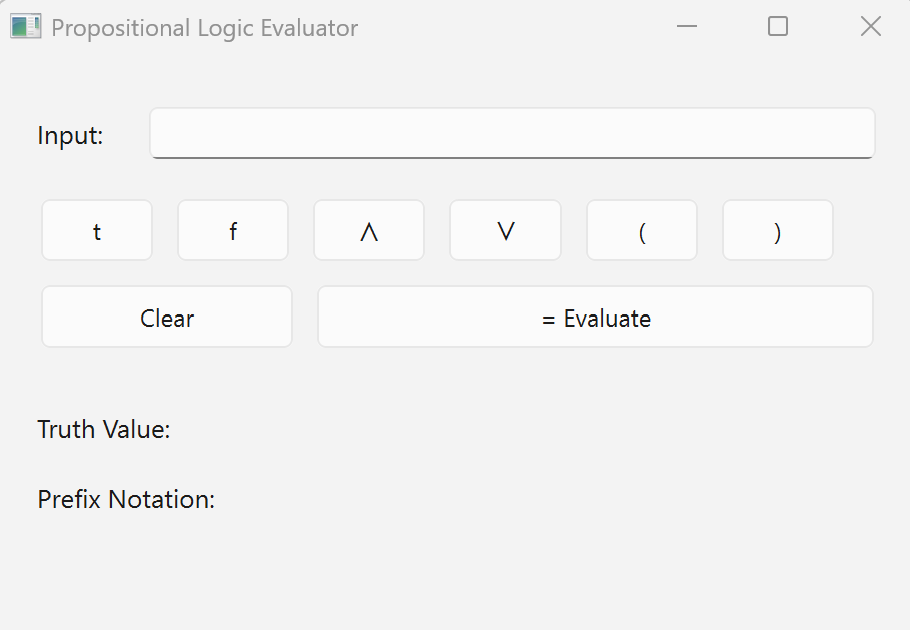
\includegraphics[width=\textwidth]{gui-preview.png}
    \caption{Empty GUI on launch}
    \label{fig:gui_preview}
\end{subfigure}
\hfill
\begin{subfigure}[t]{0.48\textwidth}
    \centering
    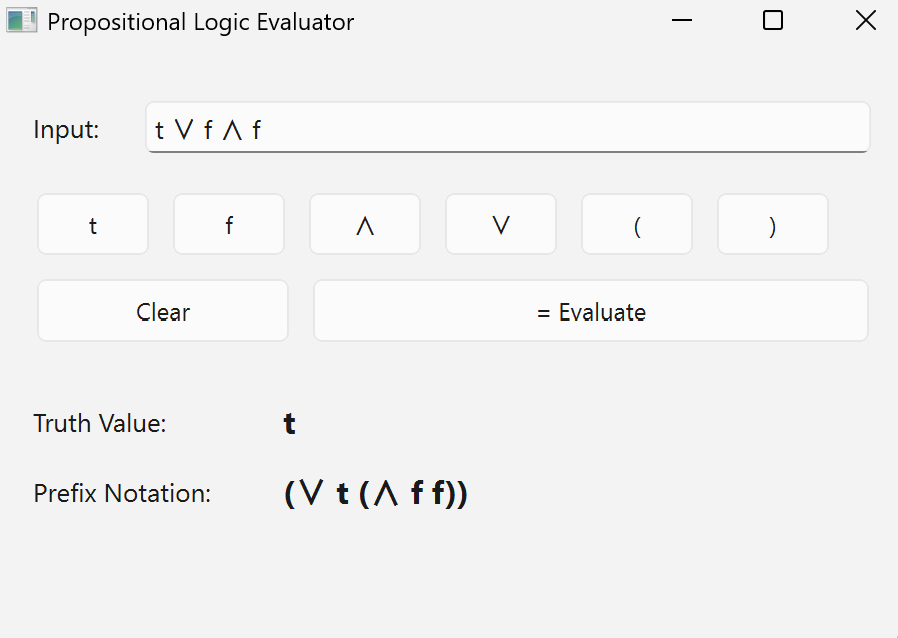
\includegraphics[width=\textwidth]{order-precedence.png}
    \caption{Operator precedence: \texttt{t $\vee$ f $\wedge$ f $\Rightarrow$ t}}
    \label{fig:order_precedence}
\end{subfigure}

\vspace{0.5em}

\begin{subfigure}[t]{0.48\textwidth}
    \centering
    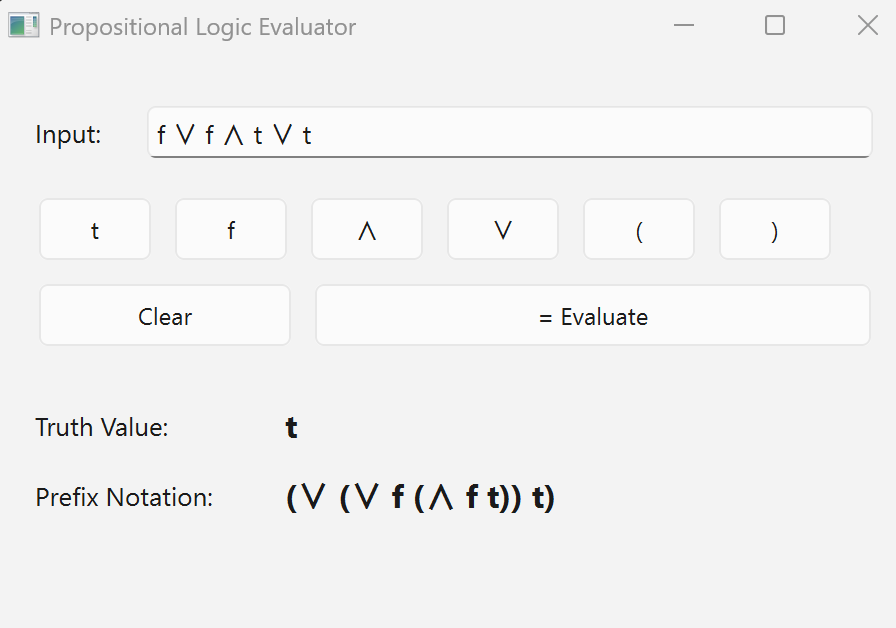
\includegraphics[width=\textwidth]{precedence-leftassoc.png}
    \caption{Left-associativity: \texttt{f $\vee$ f $\wedge$ t $\vee$ t $\Rightarrow$ t}}
    \label{fig:precedence_leftassoc}
\end{subfigure}
\hfill
\begin{subfigure}[t]{0.48\textwidth}
    \centering
    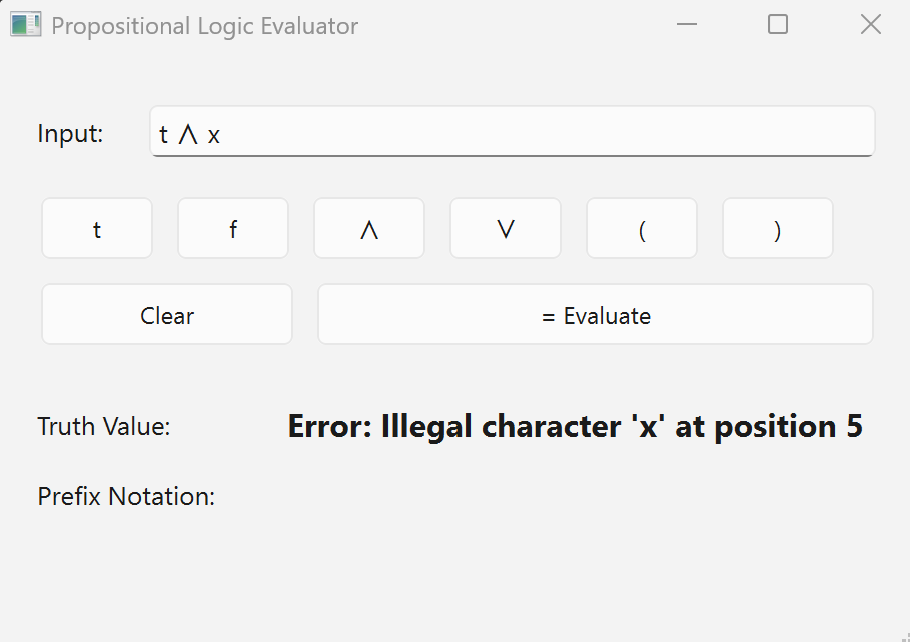
\includegraphics[width=\textwidth]{error-illegalchar.png}
    \caption{Error handling: illegal character \texttt{x}}
    \label{fig:error_illegalchar}
\end{subfigure}
\caption{Application screenshots --- GUI layout, operator precedence, left-associativity, and error handling}
\label{fig:screenshots}
\end{figure}

\subsection{GUI Interaction Flow}

When the user clicks \textbf{Evaluate}, a fresh lexer and parser are instantiated. The input text is tokenised, parsed into an AST, and the AST's \texttt{run()} and \texttt{prefix()} methods produce the truth value and prefix string, respectively.  If the input is invalid, an error message is displayed instead.


\section{Integration of Parser and Translation}

The assignment requires both a truth value and a prefix notation string from a single input.  Rather than embedding computation inside grammar rules, this implementation uses the AST as an \textbf{intermediate representation} that decouples parsing from downstream processing:

\begin{enumerate}
    \item \textbf{Parser $\rightarrow$ AST:} Each grammar rule's semantic action (Listing~\ref{lst:grammar_rules}) constructs an AST node during bottom-up reduction --- a form of \emph{syntax-directed translation}~\citep{aho2006compilers}.
    \item \textbf{AST $\rightarrow$ Truth value:} \texttt{run()} performs a post-order traversal (Listing~\ref{lst:run}).
    \item \textbf{AST $\rightarrow$ Prefix string:} \texttt{prefix()} performs a pre-order traversal (Listing~\ref{lst:prefix}).
\end{enumerate}

Because both traversals operate on the \emph{same} tree, the expression is parsed only once:

\begin{lstlisting}[caption={Pipeline integration in \texttt{MainWindow.evaluate()}}, label={lst:integration}]
result = parser.parse(lexer.tokenize(input_text))  # parse once
truth_value = result.run()                          # traversal 1
prefix_str  = result.prefix()                       # traversal 2
\end{lstlisting}

This clean separation means adding a new output format (e.g.\ postfix notation) requires only a new traversal method --- the parser and grammar remain unchanged.
